\documentclass[tikz,border=15pt]{standalone}
\usetikzlibrary{positioning, shapes.geometric, arrows.meta}

% Underline helper for primary keys
\newcommand{\pk}[1]{\underline{#1}}

\begin{document}
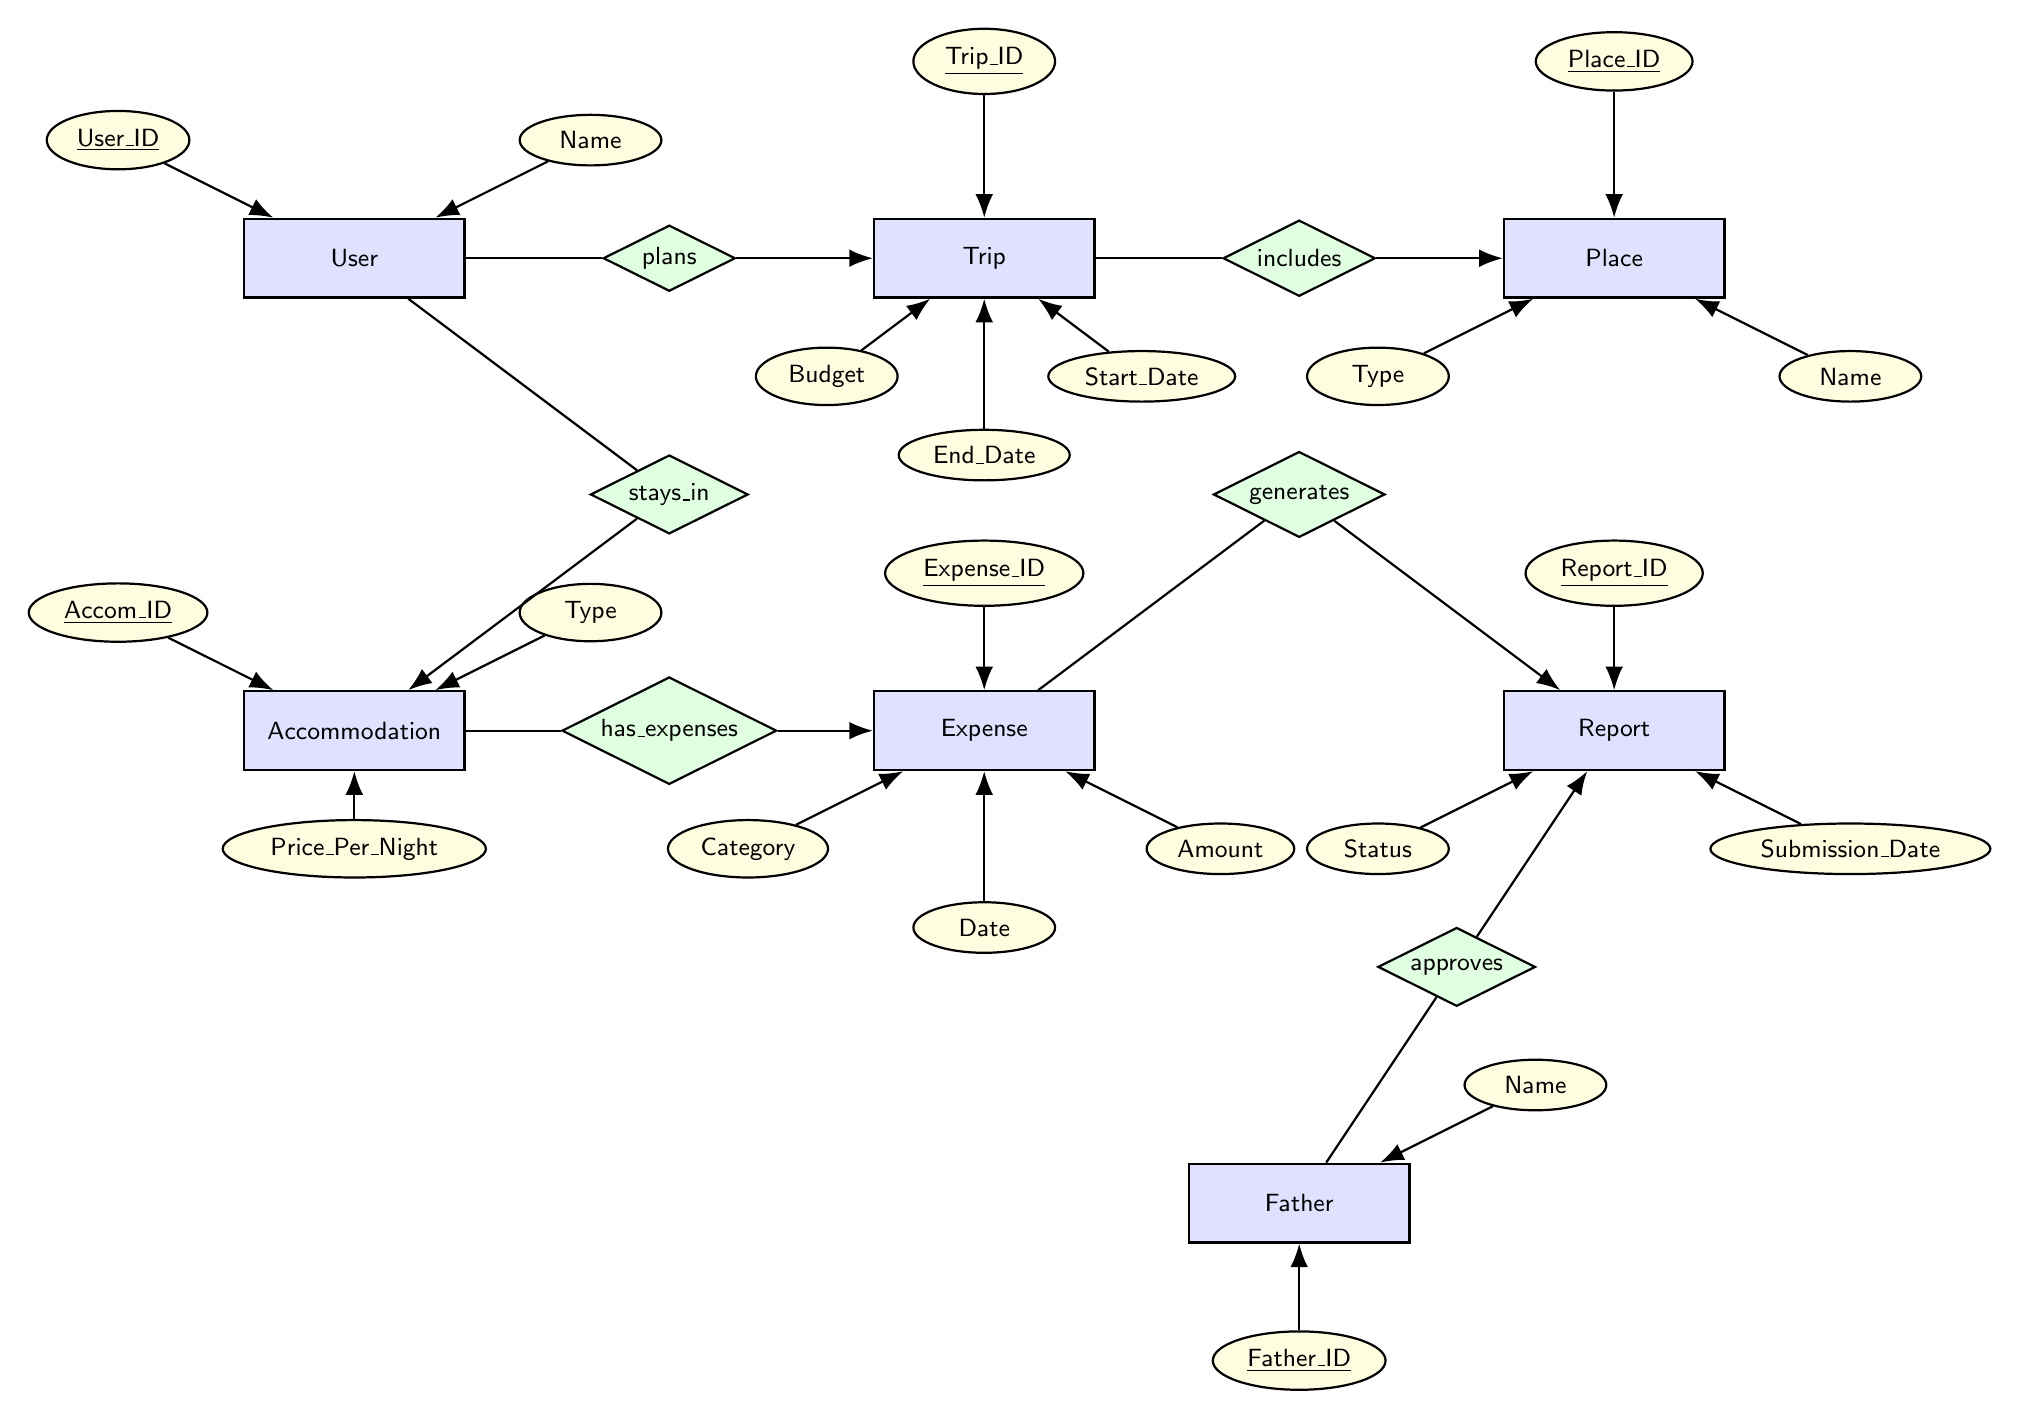
\begin{tikzpicture}[node distance=35mm and 50mm, every node/.style={font=\sffamily\small}]
  % Styles
  \tikzset{
    entity/.style = {draw, shape=rectangle, thick, minimum width=28mm, minimum height=10mm, fill=blue!12},
    relationship/.style = {draw, shape=diamond, thick, aspect=2, inner sep=2pt, fill=green!12},
    attribute/.style = {draw, shape=ellipse, thick, minimum width=18mm, minimum height=6mm, fill=yellow!12},
    link/.style = {-{Latex[length=3mm]}, thick}
  }

  % Entities
  \node[entity] (User) at (0,12) {User};
  \node[entity] (Trip) at (8,12) {Trip};
  \node[entity] (Place) at (16,12) {Place};
  
  \node[entity] (Accommodation) at (0,6) {Accommodation};
  \node[entity] (Expense) at (8,6) {Expense};
  \node[entity] (Report) at (16,6) {Report};
  
  \node[entity] (Father) at (12,0) {Father};

  % Relationships
  \node[relationship] (plans) at (4,12) {plans};
  \node[relationship] (includes) at (12,12) {includes};
  \node[relationship] (staysin) at (4,9) {stays\_in};
  \node[relationship] (hasexp) at (4,6) {has\_expenses};
  \node[relationship] (generates) at (12,9) {generates};
  \node[relationship] (approves) at (14,3) {approves};

  % User attributes
  \node[attribute] (UserID) at (-3,13.5) {\pk{User\_ID}};
  \node[attribute] (UserName) at (3,13.5) {Name};
  
  % Trip attributes  
  \node[attribute] (TripID) at (8,14.5) {\pk{Trip\_ID}};
  \node[attribute] (Budget) at (6,10.5) {Budget};
  \node[attribute] (StartDate) at (10,10.5) {Start\_Date};
  \node[attribute] (EndDate) at (8,9.5) {End\_Date};
  
  % Place attributes
  \node[attribute] (PlaceID) at (16,14.5) {\pk{Place\_ID}};
  \node[attribute] (PlaceType) at (13,10.5) {Type};
  \node[attribute] (PlaceName) at (19,10.5) {Name};
  
  % Accommodation attributes
  \node[attribute] (AccomID) at (-3,7.5) {\pk{Accom\_ID}};
  \node[attribute] (AccomType) at (3,7.5) {Type};
  \node[attribute] (PriceNight) at (0,4.5) {Price\_Per\_Night};
  
  % Expense attributes
  \node[attribute] (ExpenseID) at (8,8) {\pk{Expense\_ID}};
  \node[attribute] (Category) at (5,4.5) {Category};
  \node[attribute] (Amount) at (11,4.5) {Amount};
  \node[attribute] (EDate) at (8,3.5) {Date};
  
  % Report attributes
  \node[attribute] (ReportID) at (16,8) {\pk{Report\_ID}};
  \node[attribute] (RStatus) at (13,4.5) {Status};
  \node[attribute] (RDate) at (19,4.5) {Submission\_Date};
  
  % Father attributes
  \node[attribute] (FatherID) at (12,-2) {\pk{Father\_ID}};
  \node[attribute] (FatherName) at (15,1.5) {Name};

  % Connections
  \draw[link] (User) -- (plans) -- (Trip);
  \draw[link] (Trip) -- (includes) -- (Place);
  \draw[link] (User) -- (staysin) -- (Accommodation);
  \draw[link] (Accommodation) -- (hasexp) -- (Expense);
  \draw[link] (Expense) -- (generates) -- (Report);
  \draw[link] (Father) -- (approves) -- (Report);

  % Attribute connections
  \draw[link] (UserID) -- (User);
  \draw[link] (UserName) -- (User);

  \draw[link] (TripID) -- (Trip);
  \draw[link] (Budget) -- (Trip);
  \draw[link] (StartDate) -- (Trip);
  \draw[link] (EndDate) -- (Trip);

  \draw[link] (PlaceID) -- (Place);
  \draw[link] (PlaceType) -- (Place);
  \draw[link] (PlaceName) -- (Place);

  \draw[link] (AccomID) -- (Accommodation);
  \draw[link] (AccomType) -- (Accommodation);
  \draw[link] (PriceNight) -- (Accommodation);

  \draw[link] (ExpenseID) -- (Expense);
  \draw[link] (Category) -- (Expense);
  \draw[link] (Amount) -- (Expense);
  \draw[link] (EDate) -- (Expense);

  \draw[link] (ReportID) -- (Report);
  \draw[link] (RStatus) -- (Report);
  \draw[link] (RDate) -- (Report);

  \draw[link] (FatherID) -- (Father);
  \draw[link] (FatherName) -- (Father);

\end{tikzpicture}
\end{document}
